\chapter{Stochastic Processes and Their Simulation}

In financial engineering simulation tools have been increasingly gaining rimportance due to both the continuous enhancement of computational efficiency and the development of very complex financial, especially derivative, instruments. In this Chapter some practical applications are shown.

\section{Markov Process}

A stochastic or random process can be defined as a collection of random variables that is indexed by some mathematical set (usually time), meaning that each random variable of the stochastic process is uniquely associated with an element in the set (e.g. a time). Figure~\ref{fig:random_process} shows a graphical representation of a random process.

\begin{figure}[htb]
	\centering
	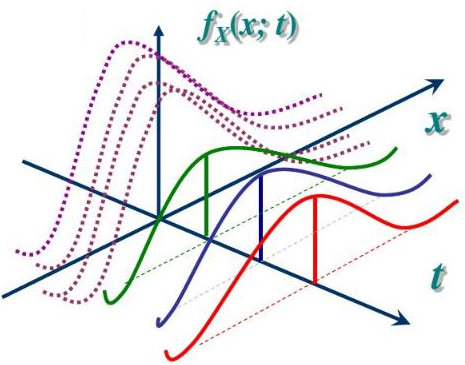
\includegraphics[width=0.5\textwidth]{figures/random_process}
	\caption{Representation of the random process $f(x, t)$. Notice how at each time $t$ it is made of different random variables $x$, each with its peculiar PDF.}
	\label{fig:random_process}
\end{figure}

A model of the dynamics of asset prices must reflect the random nature of price movements. Stock prices are usually assumed to follow a so called \emph{Markov process}. Markov processes can be characterized as a particular type of stochastic processes without any history. Past values and the way the present has emerged from the past are therefore irrelevant. This unique characteristic of Markov processes render them memoryless.

The simplest example of Markov stochastic process is the so called \emph{Wiener process} ($W$) or elementary Brownian motion, which is characterized by stationary and independent increments that are normally distributed. Those increments can be expressed as

\begin{equation}
\Delta W = Z\sqrt{\Delta t}
\end{equation}
where $Z ∼ \mathcal{N}(0, 1)$ and $\mathcal{N}$ represents the standard normal Gaussian. 
The mean of $\Delta W$ is zero and its variance is $\Delta t$, which means the standard deviation grows with the square root of time. It follows that $W(t) ∼ \mathcal{N}(0, t)$ because each $\Delta W$ is distributed like independent standard Gaussian. Figure~\ref{fig:wiener_process} shows two examples of Wiener processes.

\begin{figure}[htb]
	\centering
	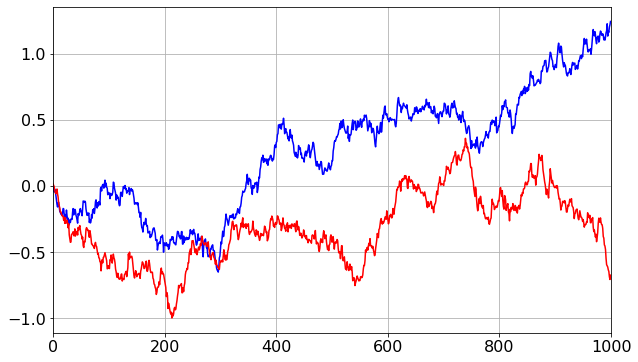
\includegraphics[width=0.7\linewidth]{figures/wiener_process.png}
	\caption{Two examples of Wiener processes.}
	\label{fig:wiener_process}
\end{figure}

An It$\hat{o}$ process ($X$) is a stochastic process whose increments satisfy the following \emph{stochastic differential equation} (SDE) 
\begin{equation}
dX(t) = \mu(t, X(t)) dt + \sigma(t, X(t)) dW(t)
\end{equation}
(notice how we moved to infinitesimal variations in the limit $\Delta t\rightarrow 0$).

In the special case where the \emph{drift} $\mu$ and the diffusion coefficient $\sigma$ are deterministic and independent of both the time $t$ and the variable $X$, the process $X(t)$ is called an \emph{arithmetic Brownian motion}. The corresponding SDE is
\begin{equation}
dX(t) = \mu dt + \sigma dW(t) = \mu dt + \sigma \sqrt{t} \mathcal{N}(0,1) 
\end{equation}
thus $X(t) ∼ \mathcal{N}(\mu t, \sigma^2 t)$.

Since an arithmetic Brownian motion can also take negative values, this type of process is apparently unsuitable for simulating asset prices. These are rather assumed to follow a \emph{geometric Brownian motion} (GBM) instead, which is going to be described in the Section. 

\section{Derivation of log-normal Stochastic Differential Equation}
\label{derivation-of-log-normal-stochastic-differential-equation}

In this Section we will see how to implement the simulation of a stock price which deviates from a steady state as a result of random fluctuations given by the trades. 

Considering a stock with a price \(S_t\) and its expected rate of return \(\mu\); the relative change in its price during a period \(dt\) can be decomposed in two parts

\begin{itemize}
	\tightlist
	\item
	a deterministic part: that is the expected return from the stock held
	during the time period \(dt\) and which can be expressed as \(\mu S_tdt\)
	\item
	a stochastic part: which reflects the random changes of the market
	(e.g. as a response to external effects such as unexpected news). A
	reasonable assumption is to take this contribution proportional to the
	stock so \(\sigma S_t dW_t\), where \(dW_t\) is a Wiener process.
\end{itemize}
Putting the two contributions together the resulting SDE is:

\begin{equation}
dS_t = \mu S_t dt + \sigma S_t dW_t
\label{eq:differential}
\end{equation}
or dividing by $S_t$
\begin{equation}
\frac{dS_t}{S_t} = d\textrm{log}(S_t) = \mu dt + \sigma dW_t
\label{eq:differential_relative}
\end{equation}

The solution of this equation can be derived by applying It\(\hat{o}\)'s formula~\cite{bib:ito_lemma}, which roughly speaking says that the derivative of a stochastic function with respect to time has an additional \emph{deterministic} term with respect to the usual derivative we know from standard calculus. 

More formally it states that for any given continuous and differentiable function \(G(S, t)\) where \(S\) satisfies the following stochastic differential equation \(dS=a\cdot dt +b\cdot dW_t\) holds

\begin{equation}
dG = \big(a\frac{\partial G}{\partial S} + \frac{\partial G}{\partial t} + \frac{1}{2}b^2\frac{\partial^2 G}{\partial S^2} \big)dt + b \frac{\partial G}{\partial S}dW
\label{eq:itos_lemma}
\end{equation}
which is essentially an extension of the Taylor series expansion for deterministic functions applicable to stochastic functions.

\begin{attention}
\subsubsection{Derivation of It$\hat{o}$'s Lemma}
Assume $X_t$ is an It$\hat{o}$ process that satisfies the stochastic differential equation
\begin{equation*}	
dX_{t}=\mu_{t}\,dt+\sigma_{t}\,dW_{t}
\end{equation*}
where $W_t$ is a Wiener process. If $f(x, t)$ is a twice-differentiable scalar function, its expansion in a \emph{Taylor series} is
	
\begin{equation*}
df={\frac {\partial f}{\partial t}}\,dt+{\frac {\partial f}{\partial x}}\,dx+{\frac {1}{2}}{\frac {\partial ^{2}f}{\partial x^{2}}}\,dx^{2}+\cdots 
\end{equation*}

Substituting $X_t$ for $x$ and therefore $\mu_t dt + \sigma_t dW_t$ for $dx$ gives
	
\begin{equation*}
df={\frac {\partial f}{\partial t}}\,dt+{\frac {\partial f}{\partial x}}(\mu _{t}\,dt+\sigma _{t}\,dW_{t})+{\frac {1}{2}}{\frac {\partial ^{2}f}{\partial x^{2}}}\left(\mu _{t}^{2}\,dt^{2}+2\mu _{t}\sigma _{t}\,dt\,dW_{t}+\sigma _{t}^{2}\,dW_{t}^{2}\right)+\cdots 
\end{equation*}

In the limit $dt\rightarrow 0$, the terms $dt^2$ and $dt\cdot dW_t$ tend to zero faster than $dW_t^2$, which is $O(dt)$. Neglecting those terms, substituting $dt$ for $dW_t^2$ (it is a Wiener process), and collecting the $dt$ and $dW_t$ terms, we obtain
	
\begin{equation*}
df=\left({\frac {\partial f}{\partial t}}+\mu _{t}{\frac {\partial f}{\partial x}}+{\frac {\sigma _{t}^{2}}{2}}{\frac {\partial ^{2}f}{\partial x^{2}}}\right)dt+\sigma _{t}{\frac {\partial f}{\partial x}}\,dW_{t}
\end{equation*}
\end{attention}
If we set \(G = \textrm{log}(S_t)\) we can compute the derivatives:

\begin{equation}
\begin{gathered}
\frac{\partial G}{\partial S} = \frac{1}{S_t}\\
\frac{\partial G}{\partial t} = 0\\
\frac{\partial^2 G}{\partial S^2} = -\frac{1}{S_t^{2}}
\end{gathered}
\end{equation}
Substituting back into Eq.~\ref{eq:itos_lemma} and taking the values of $a$ and $b$ from Eq.~\ref{eq:differential} we get:

\begin{equation}
\begin{gathered}
d(\textrm{log} S_t) = \big(\mu S_t \cfrac{1}{S_t} + \cfrac{1}{2}\sigma^2 S_t^2 (-\cfrac{1}{S_t^2})\big)dt + \sigma Z\sqrt{dt}\\
d(\textrm{log} S_t) = \textrm{log} (S_t) - \textrm{log} (S_{t-1}) = \textrm{log} \cfrac{S_t}{S_{t-1}} = \big(\mu - \cfrac{1}{2}\sigma^2\big)dt + \sigma z\sqrt{dt}\\
S_t = S_{t-1}e^{\big(\mu - \cfrac{1}{2}\sigma^2\big)dt + \sigma Z\sqrt{dt}}
\end{gathered}
\label{eq:gbm_solution}
\end{equation}
As can be seen from the following equation:

\begin{equation}
d(\textrm{log} S_t) = \big(\mu - \cfrac{1}{2}\sigma^2\big)dt + \sigma Z\sqrt{dt}
\end{equation}
the change in \(\textrm{log} S_t\) has a constant \emph{drift} with respect to time \(\mu - \frac{1}{2}\sigma^2\) and a constant variance rate \(\sigma^2\) (remember that $Z$) is a normally distributed random variable \(\mathcal{N}(0,1)\)). So you have a constant plus a Gaussian
distributed variable, therefore \(\textrm{log} S_t\) at some time \(T\) is normally distributed with:

\begin{equation}
\textrm{log}S_t - \textrm{log}S_0 \approx\mathcal{N}\big[\big(\mu-\frac{\sigma^2}{2}\big)T, \sigma^2 T\big]
\end{equation}

This equation shows that \(\textrm{log}S_t\) is normally distributed, and \textbf{such a variable whose logarithm is normally distributed is said to be log-normal}. 

The model we have just developed implies that the stock price at time T, given today's price, is log-normally distributed. One of the nicer properties of a log-normal distribution is to be positive definite and that's why log-normality is an important characteristic for stole prices: we need to \emph{ensure} that will never be negative. 

Actually this result was expected, in fact looking at the initial \(dS\) equation (Eq.~\ref{eq:differential}) we had:

\begin{equation}
dS_t = \mu S_tdt + \sigma S_t dW_t
\end{equation}
which shows that the closer \(S_t\) is to 0, the smaller is its variation \(dS\), so it will never go negative.

\section {Simulating Stochastic Differential Equations}
If we need to simulate SDEs in order to estimate quantities of interest several kinds of numerical schemes can be used. However, we restrict our discussion to the two most fundamental methods, the \emph{Euler scheme} and the \emph{Milstein scheme}. 

As a starting point for both methods, we firstly consider an SDE of the form
\begin{equation}
dX(t) = \mu(t, X(t))dt + \sigma(t, X(t)) dW (t)
\label{eq:sde}
\end{equation}

Note that both the drift $\mu$ and the diffusion $\sigma$ are functions of the process variable $X$ and the time $t$. Suppose that we are interested in simulating values of $X(T)$ without knowing its distribution. A possible reasons for that is that that Eq.~\ref{eq:sde} is simply not solvable and therefore one is not able to find an explicit solution for $X(T)$.

%Keep in mind that when we are simulating an SDE, we are actually simulating a 
%discretized version of an SDE. Therefore, a general hat notation $\hat{X}$ 
%is introduced to indicate that $\hat{X}$ is a time-discretized approximation of %the true value $X$.

\subsection{Euler Scheme}
The Euler scheme is the simplest and probably most common discretization scheme available. We generally simulate a discretized process, $\{X_b, X_{2b},\ldots, X_{mb}\} = \{X(t_i), X(t_{i+1}),...,X(t_{i+n})\}$, where the time steps $\Delta t$ are constant and denoted by $b$. Furthermore, the variable $m$ indicates the total number of simulated time steps, while $mb = T$.

Taking these preliminary considerations into account, the Euler scheme is given by
\begin{equation}
X(t_{i+1}) = X(t_i) + \mu(t_i , X(t_i))b + \sigma(t_i , X(t_i))\sqrt{b}Z_{i+1}
\label{eq:euler_scheme}
\end{equation}
where $Z_i$ are independent standard normal random vectors, $Z_i ∼ \mathcal{N}(0,I)$. 
The implementation of this method is straightforward, at least if the drift and the diffusion are easy to evaluate.

\begin{attention}
\subsection{Milstein Scheme}
The accuracy of numerical solutions of ordinary differential equations may often be improved by simple Taylor expansions. A very similar strategy also applies to SDEs. Yet it is crucial to account for the rules of It$\hat{o}$ calculus in order to maintain consistency.

Inspecting the Euler scheme~\ref{eq:euler_scheme} from the perspective of Taylor expansions leads to a possible inconsistency: running a Taylor approximation expands the drift to the order $O(b)$ but the diffusion term only to $O(\sqrt{b})$. This suggests that we focus on the diffusion term in order to advance the Euler scheme. And exactly there the Milstein scheme is applied.

The Milstein scheme is defined as an ordinary Euler scheme where the next order terms of the It$\hat{o}$-Taylor expansion of Equation~\ref{eq:sde} are additionally included. This eventually leads to

\begin{equation}
\begin{aligned}
X(t_{i+1})= X(t_i) &+ \mu(t_i, X(t_i))b+\sigma(t_i,X(t_i))\sqrt{b}Z_{i+1} \\
&+\cfrac{1}{2}\sigma'(t_i ,X(t_i))\sigma (t_i ,X(t_i))b(Z^2_{i+1} −1)
\end{aligned}
\end{equation}

The Milstein approximation thus simply involves the addition of a term to the Euler scheme so that both the drift and diffusion terms are expanded to $O(b)$ in order to eliminate the inconsistency. The Milstein scheme therefore provides a refinement of the Euler scheme based on expanding the 
diffusion term to $O(b)$ rather than just $O(\sqrt{b})$.

However, the question remains whether it is of great difference if one applies Euler’s or Milstein’s approximation for a particular diffusion equation. 

In conclusion, the approximations turn out to be very close in many simple cases. In more sophisticated models, the Milstein scheme appears to be a little better, which may be the additional benefit of the increased complexity. Of course, the two approximations do not differ at all if the diffusion coefficient $\sigma (t,X(t))$ does not depend on $X(t)$.
\end{attention}

\subsection{Simulation of a Stock Price}
%Note that the left-hand side of Eq.~\ref{eq:differential_relative} represents the 
%proportional change in the asset price in the interval $(t, t + dt)$ and additionally shows that $dS/S ∼ \mathcal{N}(\mu dt, \sigma^2 dt)$. 

Equation~\ref{eq:gbm_solution} allows us to simulate an arbitrary number of possible asset price paths by Monte Carlo. Particularly, a random path for an asset price can be simulated by sampling repeatedly for $Z$ from $\mathcal{N}(0,1)$ and substituting in Eq.~\ref{eq:gbm_solution}. 

\begin{ipython}
from numpy.random import normal, seed
from matplotlib import pyplot as plt
import math

#initial price
S = 100
mu = -0.01
sigma = 0.05
T=1
seed(1)
historical_series = [S]

# 30 days simulation
for i in range(30):
    S = S * math.exp((mu - 0.5 * sigma * sigma) * T +
                      sigma * math.sqrt(T) * normal())
    historical_series.append(S)
\end{ipython}

It is important to note that both $\mu$ and $\sigma$ are rates (variation in unit of time) that refers to the $\Delta t$ used in the simulation. In other words if $\Delta t = 1~\textrm{day}$ then the two parameters should represents the daily variations of the stock price. Figure~\ref{fig:stock_price_sim} shows possible asset price paths that are assumed to follow a geometric Brownian motion. 

\begin{figure}[htb]
	\centering
	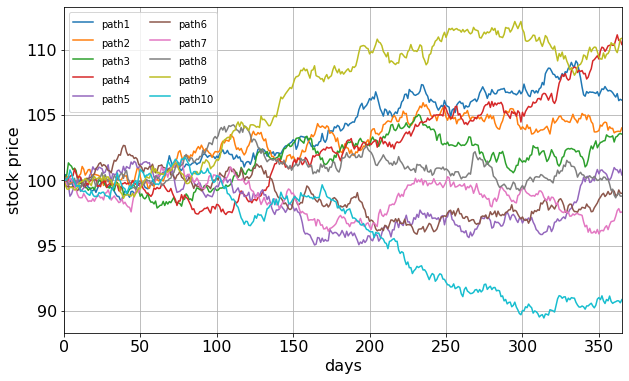
\includegraphics[width=0.7\textwidth]{figures/asset_price_simulation}
	\caption{Simulation with Monte Carlo method of three possible realization of a stock price, using geometric Brownian motion.}
	\label{fig:stock_price_sim}
\end{figure}

\subsection{Pricing Vanilla European Options by Monte Carlo}
Monte Carlo simulation fits particularly well to the pricing of a derivative. In the risk-neutral world indeed the price of a derivative can be expressed as

\begin{equation}
V(S, t) = e^{-r(T-t)} \mathbb{E}[\textrm{payoff}(S_t)]
\end{equation}
So we need to simulate different stock paths, calculate the average of the corresponding payoffs (i.e. the expectation), and discount.

%Having generated the sample paths of asset prices under the assumption of a 
%certain diffusion process, is quite easy to implement the pricing of
%derivative instruments using Monte Carlo. 
%
%A price of derivatives is eventually a function of the underlying 
%asset's price and time. Applying It$\hat{o}$'s
%lemma, we can calculate the stochastic process followed by a function
%whose inputs come from the stochastic process followed by the underlying
%itself.

Let's consider the application of Monte Carlo to a vanilla European call option. This may seem a little pointless, as there is the Black-Scholes formula which provides an analytical method that delivers the true option price much easier. Nevertheless, it builds a good and easy introduction to identify the exact Monte Carlo procedure. 

The payoff of a call option with strike $K$ and duration $T$ is 

\begin{equation}
(S(T)−K)^+ = \textrm{max}\{0,S(T)−K\}
\end{equation}

By multiplying this payoff by a discount factor $e^{−rT}$ we get the present value of the payoff. 
The expected present value and thus the call option price $C$ is defined by

\begin{equation} 
C = e^{−rT} \mathbb{E}[(S(T) −K)^+ ]
\label{eq:call_payoff}
\end{equation}

However, without the knowledge of any distributional characteristics of the random variable $S(T)$, this expectation is totally meaningless. It is impossible to price an option without any information about the distribution of its underlying price or its return. Therefore, we necessarily need to specify the particular distribution of the final asset price $S(T)$. 

In the previous Section a model for the dynamics of stock prices, namely the geometric Brownian motion, was introduced. This model provides us with the log-normal distribution of $S(T)$, the required information for a successful option pricing via expected values. Since we are in a risk-neutral environment, the drift parameter $\mu$ in Eq.~\ref{eq:gbm_solution} may be replaced by the risk-free rate $r$. Hence it is straightforward to find the asymptotically correct value for the European call option by Monte Carlo simulation. 

In a first step, simulate one path for the asset price as it is done before and calculate, according to Eq.~\ref{eq:call_payoff}, the corresponding payoff. Secondly, repeat this first step numerous times which provides you with several payoffs. Third and last step, compute the mean of the risk-free discounted payoff. 

The fact that this Monte Carlo estimate is indeed consistent with the Black-Scholes formula results is illustrated in Fig.~\ref{fig:error_BS}. It shows the development of the relative pricing error, computed as $(C_n − C)/C$, with a steadily growing sample $n$. Note that the pricing error is gradually decreasing and eventually converging to 0 as $n$ goes to infinity. This is another proof that Monte Carlo provides correct results in the limit $n\rightarrow\infty$.

\begin{figure}[htb]
	\centering
	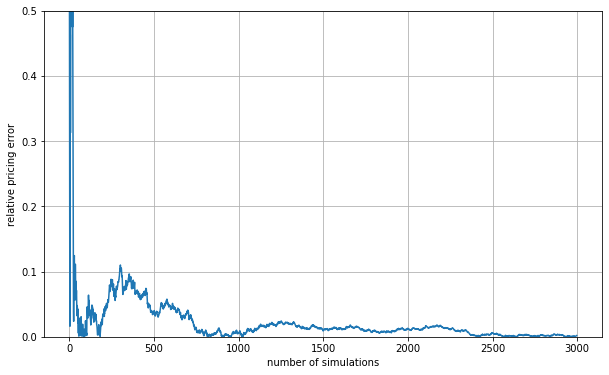
\includegraphics[width=0.7\textwidth]{figures/call_pricing_error.png}
	\caption{Development of the relative pricing error for a call between MC simulation and BS formula with growing samples.}
	\label{fig:error_BS}
\end{figure}

\section{Markov Chain}
\label{sec:markov_chain}
A \emph{Markov chain} is a mathematical system usually defined as a collection of random variables, that transition from one state to another according to certain probabilistic rules. These set of transition satisfies the Markov property, which states that the probability of transitioning to any particular state is dependent solely on the current state and time elapsed, and not on the sequence of state that preceded it. 

Markov Chains have prolific usage in mathematics. They are widely employed in economics, game theory, communication theory, genetics and finance. They arise broadly in statistics (specially Bayesian statistics) and information-theoretical contexts. When it comes real-world problems, they are used to postulate solutions to study cruise control systems in motor vehicles, queues or lines of customers arriving at an airport, exchange rates of currencies, etc. 

A Markov chain is then a random process and has either discrete state space (set of possible values of the random variables) or discrete index set (often representing time), given the fact, many variations for a Markov chain exists. 

\subsection{Discrete Time Markov Chain}
A discrete-time Markov chain involves a system which is in a certain state at each step, with the state changing randomly between steps. The steps are often thought of as moments in time (but you might as well refer to physical distance or any other discrete measurement). A discrete time Markov chain is a sequence of random variables $X_1, X_2, X_3,\ldots$ with the Markov property, such that the probability of moving to the next state depends only on the present state and not on the previous states. Putting this is mathematical probabilistic formula:

\begin{equation}
P(X_{n+1}) = x | X_1 = x_1, X_2 = x_2, \ldots, X_n = x_n) = P( X_{n+1} = x | X_n = x_n)
\end{equation}

The probability of $X_{n+1}$ only depends on the probability of $X_n$ that precedes it. Which means the knowledge of the previous state is all that is necessary to determine the probability distribution of the current state, satisfying the rule of conditional independence.

Some interesting properties of Markov chains are:

\begin{itemize}
	\tightlist
	\item reducibility: a Markov chain is said to be irreducible if it is possible to get to any state from any state. In other words, a Markov chain is irreducible if there exists a chain of steps between any two states that has positive probability;
	\item periodicity: a state in a Markov chain is periodic if the chain can return to the state only at multiples of some integer larger than 1. Thus, starting in state $i$, the chain can return to $i$ only at multiples of the period $k$, and $k$ is the largest such integer. State $i$ is aperiodic if $k = 1$ and periodic if $k > 1$;	
	\item transience and recurrence: A state $i$ is said to be transient if, given that we start in state $i$, there is a non-zero probability that we will never return to $i$. State $i$ is recurrent (or persistent) if it is not transient. A recurrent state is known as positive recurrent if it is expected to return within a finite number of steps and null recurrent otherwise;
	\item ergodicity: a state $i$ is said to be ergodic if it is aperiodic and positive recurrent. If all states in an irreducible Markov chain are ergodic, then the chain is said to be ergodic;
	\item absorbing state: a state $i$ is called absorbing if it is impossible to leave this state. Therefore, the state $i$ is absorbing if $t_{ii} = 1$ and $t_{ij}$ = 0 for $i \neq j$. If every state can reach an absorbing state, then the Markov chain is an absorbing Markov chain.
\end{itemize}

%The possible values of $X_i$ form a countable set $S$ called the state space of the chain. The state space can be anything: letters, numbers, basketball scores or weather conditions. While the time parameter is usually discrete, the state space of a discrete time Markov chain does not have any widely agreed upon restrictions, and rather refers to a process on an arbitrary state space. However, many applications of Markov chains employ finite or countably infinite state spaces, because they have a more straightforward statistical analysis.

\subsection{The Markov Model}
A Markov chain can be represented by a set of probabilities associated with the various possible transitions (the changes of state of the system). These probabilities are usually put in matricial form creating the \emph{transition matrix}.
Each element of the matrix $P(X_{n+1} = x | X_n = x_n)$ can be read as the probability of going to state $X_{n+1}$ given the current value of state $X_n$. The same information is represented by the transition matrix from time $n$ to time $n+1$.

If the Markov chain has $N$ possible states, the matrix will be an $N \times N$ matrix, such that entry $(i, j)$ is the probability of transitioning from state $i$ to state $j$. Additionally, the transition matrix must be a \emph{stochastic matrix}, a matrix whose entries in each row must add up to exactly 1, since each row represents its own probability distribution.

So, the model is characterized by a state space (the set of possible state of the system), a transition matrix describing the probabilities of particular transitions, and an initial state across the state space. Let's work out a real example. 

\subsection{Markov Chain to Predict Market Trends}
Markov chains and their respective diagrams can be used to model the probabilities of certain
financial market climates and thus predicting the likelihood of future market conditions.
These conditions, also known as trends, are:
\begin{itemize}
\item bull markets: periods of time where prices generally are rising, due to the actors
having optimistic hopes of the future;
\item bear markets: periods of time where prices generally are declining, due to the actors
having a pessimistic view of the future;
\item stagnant markets: periods of time where the market is characterized by neither a
decline nor rise in general prices.
\end{itemize}

In fair markets, it is assumed that market information is distributed equally among its actors and that prices fluctuate randomly. This means that every actor has equal access to information such that no actor has an upper hand due to inside-information. Through technical analysis of historical data, certain patterns can be found as well as their estimated probabilities. For example, consider a hypothetical market with Markov properties where historical data has given us the patterns depicted in Fig.~\ref{fig:markov_chain}.
After a week characterized of a \emph{bull market} trend there is a 90\% chance that another bullish week will follow. Additionally, there is a 7.5\% chance that the bull week instead will be followed by a bearish one, or a 2.5\% chance that it will be a stagnant one. Similarly for the other states. 

\begin{figure}[htb]
	\centering
	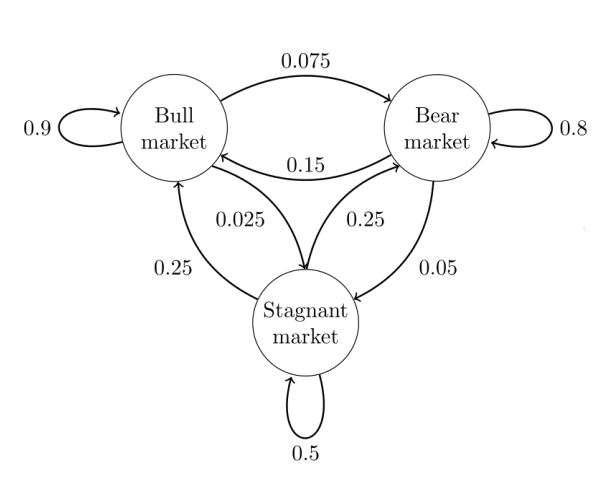
\includegraphics[width=0.7\textwidth]{figures/markov_chain}
	\caption{Graph showing the transition probabilities between three weekly market states: bull, bear and stagnant.}
	\label{fig:markov_chain}
\end{figure}

By compiling these probabilities into a table, it is easy to derive the transition matrix $\Pi$

\[\Pi = 
\begin{bmatrix}
p_{11} & p_{12} & p_{13} \\
p_{12} & p_{22} & p_{23} \\
p_{13} & p_{32} & p_{33}
\end{bmatrix} =
\begin{bmatrix}
0.9 & 0.075 & 0.025 \\
0.15 & 0.8 & 0.05 \\
0.25 & 0.25 & 0.5
\end{bmatrix} 
\]

Let's indicate with a $1 \times 3$ vector $C$ the information about which of the three different states any current week the market is in; where column 1 represents a bull week, column 2 a bear week and column 3 a stagnant week. Assume that today's week the market is in a bearish state, resulting in the vector $C_0  = (0, 1, 0)$.

To calculate the probabilities of a bull, bear or stagnant week for any number of $n$ weeks into the future it is enough to multiply $C$ by the transition matrix $n$ times ($C_n = C_0\cdot \Pi^n$)

\[C_1 = C_0 \cdot \Pi =  
\begin{bmatrix}
0 \\
1 \\
0 
\end{bmatrix}
\begin{bmatrix}
0.9 & 0.075 & 0.025 \\
0.15 & 0.8 & 0.05 \\
0.25 & 0.25 & 0.5
\end{bmatrix} = 
\begin{bmatrix}
0.15 \\
0.8 \\
0.05 
\end{bmatrix}
\]

The model predicts an 80\% probability for the market to stay in a bearish mode also in the next week, 15\% to become bullish and just a 5\% to be stagnant.

With \texttt{python} it is possible to determine longer term behaviour up to the \emph{stationary distribution}. The stationary distribution is the fraction of time that the system spends in each state as the number of iterations approaches infinity.

\begin{ipython}
import numpy as np

n = 50
hist_C = np.zeros(shape=(n, 3))
C = np.array([0, 1, 0])
P = np.array([[0.9, 0.075, 0.025],[0.15, 0.8, 0.05],[0.25, 0.25, 0.5]])

for i in range(n):
    hist_C[i] = C
    C = C.dot(P)

print (C)
\end{ipython}
\begin{ioutput}
[0.62499979 0.31250019 0.06250002]
\end{ioutput}

From this example it can be concluded that as $n \rightarrow \infty$, the probabilities will converge to a steady state, meaning that 63\% of all weeks will be bullish, 31\% bearish and 6\% stagnant. Figure~\ref{fig:markov_chain_sim} reports the various probabilities at each iteration. The system converges to the stationary state after about 20 weeks.
It can also be shown, by changing $C_0$ that the steady-state probabilities of this Markov chain do not depend upon the initial state. 

\begin{figure}[!t]
	\centering
	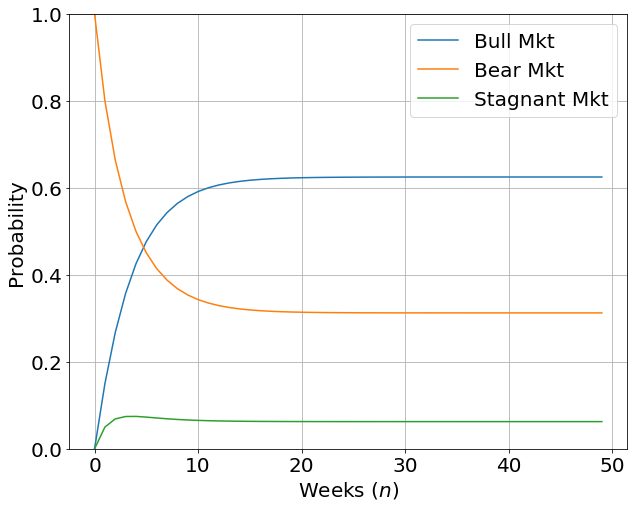
\includegraphics[width=0.7\textwidth]{figures/markov_chain_sim}
	\caption{Simulation of weekly market trend for $n=50$. The system reaches the stationary state relatively quickly after about 20 weeks.}
	\label{fig:markov_chain_sim}
\end{figure}

The results can be used in various ways, some examples are calculating the average time it takes for a bearish period to end, or the risk that a bullish market turns bearish or stagnant.

\begin{thebibliography}{9}
\bibitem{bib:stochastic_calculus} P. Wilmott, \emph{Quantitative Finance (2nd edition)}, Elementary Stochastic Calculus (Ch. 4), John Wiley and Sons, 2006 
\bibitem{bib:ito_lemma}\href{https://en.wikipedia.org/wiki/It\%C3\%B4\%27s_lemma}{\emph{It$\hat{o}$'s Lemma}}, Wikipedia [Online]
\bibitem{bib:euler_scheme} \href{https://en.wikipedia.org/wiki/Euler_method}{\emph{Euler Scheme}}, Wikipedia [Online]
\end{thebibliography}









